\documentclass[10pt]{article}

\usepackage{graphicx}
\usepackage{amsmath}
\usepackage[ansinew]{inputenc}
\usepackage[spanish]{babel}
\usepackage{babelbib}
\usepackage[T1]{fontenc}
\usepackage[vmargin=4cm,hmargin=4cm,letterpaper]{geometry}
\usepackage{color}
\usepackage{framed}
\usepackage{hyperref}

\usepackage{listings}
\definecolor{red}{RGB}{219,0,0}
\definecolor{pink}{RGB}{255,100,100}
\definecolor{gray}{RGB}{100,100,100}
\lstset{
		basicstyle=\ttfamily,
		frame=single,
		keywordstyle=\color{red},
		commentstyle=\color{gray},
		stringstyle=\color{pink},
		tabsize=3,
		language=verilog,
		backgroundcolor=\color{white}}

\usepackage{fancyhdr} 
\pagestyle{fancy}
\usepackage{lastpage}
\lhead{Laboratorio 3}
\chead{}
\rhead{Bit�cora}
\lfoot{}
\cfoot{}
\rfoot{\footnotesize Page \thepage\ of \pageref{LastPage}}

\renewcommand{\headrulewidth}{0.4pt} 
\renewcommand{\footrulewidth}{0.4pt} 

\graphicspath{{../media/}}	%%multimedia path
\setlength{\parindent}{0pt}
%%*************************************************************************
\begin{document}

\begin{huge}
\begin{center}
\textbf{Laboratorio 3: Circuitos combinatorios}
\end{center}
\end{huge}

\begin{Large}
\begin{center}
Jose Ap� (B10407), Francisco Molina (B14194), \\Marco Montero (A94000), Dennis Vargas (B16831)
\end{center}
\end{Large}


\section*{Ejercicio 1}
Implemente una m�quina de estados que permita escribir y leer datos de una memoria SRAM del Spartan 6.\\[0.3 cm]
papilio duo, tiene fpga, un wing que permite usar leds, ver que esta leyendo y escribiendo con los leds para debuggear. poner pines y comparalos con el utf.


\begin{figure}[hbtp]
\centering
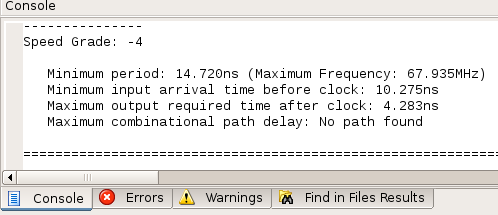
\includegraphics[width=12 cm]{../media/mul_max_freq.png}
\caption{Frecuencia m�xima del operador * sin signo}
\label{freq1}
\end{figure}

\begin{lstlisting}
wire [9:0] wA, wB;
wire [31:0] R = wA * wB; //multiplicaci�n sin signo
wire signed [15:0] wA, wB;
wire signed [31:0] wR = wA * wB; // multiplicaci�n con signo
\end{lstlisting}
Note en la figura siguiente como el simulador reconoce la multiplicaci�n con signo:




\end{document}
%%*************************************************************************
